\documentclass[11pt,a4paper]{article}
\usepackage[margin=2.4cm]{geometry}
\usepackage{amsmath,amssymb,amsthm}
\usepackage{graphicx}
\usepackage{booktabs}
\usepackage{enumitem}
\usepackage{xcolor}
\usepackage{listings}
\usepackage[colorlinks=true,linkcolor=blue!60!black,citecolor=blue!60!black]{hyperref}
\graphicspath{{../figures/}}

\newtheorem{theorem}{Theorem}[section]
\newtheorem{corollary}[theorem]{Corollary}
\newtheorem{proposition}[theorem]{Proposition}
\newtheorem{lemma}[theorem]{Lemma}
\theoremstyle{definition}
\newtheorem{definition}[theorem]{Definition}
\newtheorem{claim}[theorem]{Verified Claim}
\newtheorem{remark}[theorem]{Remark}

\lstdefinestyle{code}{basicstyle=\ttfamily\scriptsize, columns=fullflexible,
  breaklines=true, frame=single, rulecolor=\color{black!30}, aboveskip=8pt, belowskip=8pt}

\title{\textbf{Pulsar: Exact Tree Speculation with Confidence-Based Scheduling}}
\author{The Pulsar Project\\\small technical report v0.2 --- Stage 6 backend study}
\date{October 2026}

\begin{document}
\maketitle

\begin{abstract}
\noindent
Speculative decoding trades draft and verification work against the target
model's autoregressive cost. Pulsar's frozen verifier gives a pointwise
exactness guarantee: proposing from $q$, accepting with $\min(1,p/q)$, and
drawing a rejection replacement from $(p-q)_+$ preserves the target next-token
law $p$. This guarantee does not imply a throughput gain. The central empirical
hypothesis is conditional and falsifiable: under a measured backend cost
profile, a draft-confidence scheduler for exact bounded trees improves held-out
tokens/s over a tuning-selected fixed tree only if the paired 95\% confidence
interval's lower bound is positive. A Stage 6 Hugging Face Transformers CPU
integration (distilgpt2 target, tiny-gpt2 draft, temperature-1 softmax, 24-token
horizon, three held-out prompts) passed the full-vocabulary verifier identity
with maximum absolute error $1.1\cdot10^{-19}$. However, the confidence-tree
point estimate was $+1.66\%$ versus the fixed tree, with 95\% CI
$[-6.71\%,+10.01\%]$; all confidence bins selected the same fixed action, so
the scheduler claim is not established. Tuned $\gamma=2$ chain speculation
reached 15.71 tokens/s and beat the fixed tree (10.98 tokens/s) by 43.00\%
$[34.87\%,50.79\%]$, but both were slower than autoregression at 40.62
tokens/s. Earlier $1.39\times$ results are from an analytic cost-model Markov
testbed, not measured neural-model acceleration. Pulsar, rotor, and quantum
terminology is explanatory framing; those mechanisms are not part of the Stage
6 measured algorithm.
\end{abstract}

\section{Introduction}

\subsection{The emission bottleneck}
Every mainstream LLM is a decoder: each forward pass produces a distribution
over $V$ outcomes and then destroys it, emitting a single sample. The engine
pays the memory-bound per-token tax because it retains no representation of
the \emph{future field} and no principled scheduler for \emph{when} to
collapse it. Speculative decoding and its successors (Medusa, EAGLE,
Lookahead, Sequoia) draft candidate fields and verify in parallel, but the
field is handled ad hoc: fixed speculation lengths, hand-tuned acceptance
rules, and tree samplers whose renormalization quietly changes the proposal
the verifier must respect.

A pulsar is nature's solution to ``emit fast from a huge field'': a rotating
magnetized star sweeps a beam through the entire sky, observers receive
\emph{pulses} whose timing is predictable to extraordinary precision. Three
features transfer into an inference engine: (1) a \textbf{rotor sweeping a
field} --- stratified, budgeted coverage of candidates; (2) \textbf{pulses,
not streams} --- commit when local field density (confidence) crosses a
threshold, emitting $1..N$ tokens; (3) a \textbf{clock independent of
content} --- per-cycle work is bounded by construction.

\subsection{Design stance}
The novel, trainable core is deliberately \emph{sub-symbolic and small}: a
confidence field (M4c) estimating verifier-acceptance probabilities from
draft-side features. Everything correctness-critical is \emph{frozen}: the
rejection-sampling verifier guarantees that no matter how M1, M2, M4a--M4d,
M7 misbehave --- even adversarially --- output remains the base model's
distribution. Speed is bought with miscalibration; quality cannot be. This
asymmetry is what makes a fast engine shippable, and it is the paper's
organizing theorem.

\subsection{Contributions}
\begin{enumerate}[label=\textbf{C\arabic*},leftmargin=3.6em]
\item \emph{Superposition fields} (\S\ref{sec:core}): prefix-tree candidate
structures with Born-shaped path amplitudes; ``quantum'' language bounded to
diagonal density operators; the branching domain is the load-bearing object.
\item \emph{Exactness Theorem in full generality} (\S\ref{sec:exact}): verify
against the \emph{effective collapse policy}, not the raw draft --- exact for
any proposal, temperature, pruning, adversarial selector. Implies a design
correction: renormalizing proposals to kept tree children strictly lowers
acceptance; the remedy is \emph{fall-through collapse} (C4).
\item \emph{Water-level pulses, proved optimal} (\S\ref{sec:pulse}):
blocks $\{A(u)\ge\theta\}$ with self-consistent $\theta^\ast=d\,S^\ast$
maximize tokens-per-cost over all prefix-closed subtrees; brute-force
verified at slack $10^{-16}$; two online learners reach it (fixed point,
bandit).
\item \emph{Fall-through collapse} (\S\ref{sec:collapse}): the descent draws
from the draft's own law; the block only pre-decides continuation depth.
Measured vs renormalized tree sampling on identical machinery:
$1.388$ vs $1.079$ ($+29\%$), exactness preserved in both.
\item \emph{Confidence-field theory} (\S\ref{sec:conf}): the water level is
optimal iff $\mathbb E[a\mid\hat a]=\hat a$ at decision granularity ---
calibration is not cosmetic. A logistic head with PAVA isotonic reaches
$\mathrm{ECE}=7\cdot10^{-4}$, capturing $97.5\%$ of the oracle-$\hat a$
ceiling; tail-bin limits are an information ceiling, documented.
\item \emph{LIF equivalence} (\S\ref{sec:conf}): leaky accumulate-and-fire
equals the analytic pulse-timing law exactly (verified) --- the SNN reading
of M4a/M4c is a theorem under this mapping.
\item \emph{Bounds and regime maps} (\S\ref{sec:cost}):
$\alpha=1-\mathrm{TV}$, Pinsker/Bretagnolle--Huber divergence floors,
optimal block sizes, measured crossovers where speculation flips negative.
\item \emph{Verification-first artifact} (\S\ref{sec:verify}, \S\ref{sec:practice}):
Python reference, 11+21-check harness (all green), C++17 engine passing its
own acceptance test, cross-implementation agreement, and a bug log
including two errors in the tests' own references.
\end{enumerate}

\subsection{What this is not}
Not a new base model, not quantum computing, not a claim about brains or
stars computing probabilities. It is an engine discipline: module contracts,
theorems, an online calibrator, and a harness that refuses drift.

\section{Related work, in equations}
\label{sec:related}
\textbf{Speculative decoding} (Leviathan et al.\ 2023; Chen et al.\ 2023):
draft $q$ of length $\gamma$; accept with $\min(1,p/q)$; residual resampling.
Yield $\tau(\alpha,\gamma)=(1-\alpha^{\gamma+1})/(1-\alpha)$, speedup
$S=\tau/(1+c\gamma)$; 2--3$\times$ at $c\approx0.1$. Our T02/T03 re-derive
these to machine precision; E03 implements the baseline \emph{honestly}
(blind drafting cost, single verification pass).
\textbf{Medusa} (Cai et al.\ 2024): $K$ parallel heads + \emph{typical
acceptance} (accept draft tokens in the target's top-mass set), trading
exactness for acceptance volume. Pulsar keeps rejection sampling exact and
moves intelligence into \emph{which regions get pre-verified}.
\textbf{EAGLE-1/2/3} (Li et al.\ 2023--2025): autoregressive drafting in
feature space (the sub-symbolic precedent), dynamic trees by score budgets;
EAGLE-3 reports up to $6.5\times$ ($1.4\times$ over EAGLE-2) and $1.38\times$
throughput at batch 64 in SGLang (arXiv:2503.01840). Pulsar axiomatizes
EAGLE's engineering: score $=$ calibrated acceptance; budget $=$ water level
with self-consistent $\theta$; fall-through removes a proposal mismatch tree
sampling lives with. \textbf{Lookahead/prompt-lookup/Sequoia}: fixed n-gram
caches or offline-optimal trees; our rotor generalizes cyclic readout with a
variance bound, and M7 replaces tree-size heuristics with a learned scalar.
\textbf{SNNs} (Gerstner et al.): LIF thresholded accumulation; T08 proves
membrane threshold $\equiv$ pulse threshold for our dynamics.
\textbf{Block-diffusion LMs} generate several tokens jointly; Pulsar is
complementary --- it \emph{selects among} candidates, and its economics sit
on top of any M1 backend.

\section{The formal core}
\label{sec:core}
\begin{definition}[Field and amplitudes]
\label{def:field}
Let $p(\cdot\mid t_{\le n})$ be the frozen target law on $\mathcal V$,
$|\mathcal V|=V$, and $q(\cdot\mid s_n)$ a draft-side law with visible
context $s_n$. A \emph{candidate field} is a prefix tree $T$; node
$u$ carries token $x_u$, parent $\mathrm{par}(u)$, path
$x_{1..\mathrm{dep}(u)}$, and two products
\begin{equation}
\psi(u)=\!\!\prod_{v\le u}\!\! q(x_v\mid s(v))
\qquad
A(u)=\!\!\prod_{v\le u}\!\! q(x_v)\,\hat a(v),
\end{equation}
with $\hat a$ the acceptance estimate of \S\ref{sec:conf}.
A \emph{cut} is a set of nodes covering root-to-leaf paths; its frontier is
an antichain $\mathcal C$ of mutually exclusive futures. The \emph{Born
weights} $P_{\mathcal C}(u)=\psi(u)/\sum_{w\in\mathcal C}\psi(w)$ define the
collapse law over $\mathcal C$.
\end{definition}
\begin{remark}[Quantum language, bounded]
$\rho=\sum_u \psi(u)^2\,|u\rangle\langle u|$ is diagonal: no interference,
no entanglement, no hardware. All results below are elementary probability
with disciplined conditioning; the import is the branching domain and
Born-shaped weights, and the ``measurement'' is conditional resampling.
Exactness (Thm~\ref{thm:exact}) even tolerates a literal quantum sampler as
$\pi$, should one exist.
\end{remark}

\subsection{The verifier and the Exactness Theorem}
\label{sec:exact}
At each descent node the collapse draws from a \emph{policy}
$\pi_u$ --- raw $q$ (fall-through), $\mathrm{softmax}(\log q/T)$,
or a $\delta$ (greedy/adversarial). The verifier tests that exact law:
\begin{equation}
x\sim\pi_u:\quad
\text{accept } x \text{ w.p. } a(x)=\min\!\big(1,\tfrac{p(x)}{\pi_u(x)}\big),
\qquad
\text{else emit } y\sim r=\mathrm{norm}\big(\max(p-\pi_u,0)\big).
\end{equation}
\begin{theorem}[Exactness, proposal- and policy-agnostic]
\label{thm:exact}
For any law $\pi$ (any dependence on history, $\hat a$, $\theta$,
temperature; even adversarial), the emitted token is distributed exactly as
$p$, provided acceptance coins are fresh and independent of the policy.
\end{theorem}
\begin{proof}
Pointwise, with $A=\sum_x \pi\wedge p = 1-\mathrm{TV}(p,\pi)$ and
$\sum_x(p-\pi)^+=1-A$:
\[
\pi(x)a(x)+(1-A)\,r(x)=\pi\wedge p+(p-\pi)^+=p.\qquad\qedhere
\]
\end{proof}
\begin{corollary}[Yield law]
\label{cor:yield}
Sequential descent with per-position coins, stopping at first rejection,
plus a bonus token from the same pass's next row, gives per-step yields
distributed as target autoregression over the block;
$\mathbb E[\text{tokens}]=1+\sum_{k\ge1}\prod_{j\le k}\alpha_j$ with
$\alpha_j=\mathbb E[\,a\,]$; uniform $\alpha$ recovers
$\tau(\alpha,\gamma)=(1-\alpha^{\gamma+1})/(1-\alpha)$.
\end{corollary}
\begin{corollary}[Acceptance--divergence identity]
\label{cor:tv}
$\alpha(\pi)=\sum_x\pi\min(1,p/\pi)=1-\mathrm{TV}(p,\pi)$, and by Pinsker and
Bretagnolle--Huber:
$\alpha\ge 1-\sqrt{\mathrm{KL}/2}$, \
$\mathrm{TV}\le\sqrt{1-e^{-\mathrm{KL}}}$.
\end{corollary}
Verified: T01/T09/T10 (random and adversarial pairs; $\chi^2$ fit), E02
(measured acceptance vs.\ table truth, $z=-0.28/-0.13$), E01 (engine, 11
policies), C++ (250k samples).

\section{Modules: mathematics and mechanism}
\subsection{M1 generator, M2 field, M3 verifier, M5 commit}
M1: top-$B$ expansion of $q$, or any backend emitting
$(x,\log q(x))$ pairs (Medusa/EAGLE heads, retrieval) --- swappable by
contract. M2 as Definition~\ref{def:field}: branching is first-class until
measurement. M3 runs Theorem~\ref{thm:exact} along the collapsed path with
one batched tree pass computing all needed $p$-rows; M5 commits
accepted prefix $\oplus$ (residual $\mid$ bonus) and appends caches.

\subsection{M4a rotor: stratified sweep, circulant mixing}
\label{sec:rotor}
Per tick, a batch $B_t$ of field nodes is read (scored/updated) in fixed
cyclic order. Over one cycle every node is read exactly once: the readout is
\emph{sampling without replacement}, and for the field-mean estimator
\begin{equation}
\mathrm{Var}_{\text{strat}}(\bar x)=\frac{\sigma^2}{n}\cdot\frac{N-n}{N-1}
\;<\;\frac{\sigma^2}{n}=\mathrm{Var}_{\text{iid}}(\bar x).
\end{equation}
Measured ratio $0.499$ vs predicted $0.504$ (T06). Sibling evidence mixing
$M_\varepsilon=(1-\varepsilon)I+\frac{\varepsilon}{n}\mathbf 1\mathbf 1^\top$
is row-stochastic --- total Born mass preserved --- with spectrum
$\{1,(1-\varepsilon)^{n-1}\}$: a contraction only on the disagreement
subspace (a noise smoother; verified T06).

\subsection{M4c confidence field (trainable sub-symbolic core) and LIF form}
\label{sec:conf}
$\hat a(x,s)=\mathrm{iso}\big(\sigma(w\!\cdot\!\varphi(x,s)+b)\big)$ with
draft-only features
$\varphi\!=\!(1,\log q, -H(q), \log q\!-\!\log q_1, \log q_1, \mathrm{rank})$,
trained on verifier labels $\min(1,p(x)/q(x))$ by soft BCE; PAVA isotonic head
guarantees decision-granular calibration
$\mathbb E[a\mid\hat a\in\text{bin}]\approx\hat a$:
held-out $n=195{,}072$, ECE $7\cdot10^{-4}$, slope $0.9995$, max bin gap
$0.007$, median $0.0006$ (E04). Tail-bin residual error is an
\emph{information ceiling of draft-only features}: adding interaction terms
destabilized GD without closing it (documented, log V9).
\emph{LIF equivalence:} with
$V_t=(1-\lambda)V_{t-1}+\lambda e_t$ firing at $V_t\ge\theta$, constant drive
$I>\theta$ fires at exactly
$t^\ast=\lceil\ln(1-\theta/I)/\ln(1-\lambda)\rceil-1$ --- verified against
simulation on 300 random instances (T08). ``Neurons as confidence
integrators'' is a theorem here, not a metaphor.

\subsection{M4b pulse generator: water-level blocks}
\label{sec:pulse}
Given node values $A(u)$ (cumulative expected marginal tokens --- overlap
mass $\prod q\hat a$), per-node cost $d$ in target-pass units,
step cost $C=1+dN$ and yield $T=1+\sum_{u}A_{\text{true}}(u)$, latency
$L=C/T$:
\begin{theorem}[Water-level optimality]
\label{thm:water}
If $A$ decreases along paths, the prefix-closed block that maximizes $T/C$
over \emph{all} prefix-closed subtrees is the water level
$\{A(u)\ge\theta^\ast\}$, $\theta^\ast=d\,T^\ast/C^\ast=d\,S^\ast$, realized
by the greedy single-crossing scan (include while
$A_u \ge d\,T/C$ evaluated on the current set).
\end{theorem}
\begin{proof}[Proof sketch (chain; App.~A.3 for trees)]
$\Delta L(H)=L(H{+}1)-L(H)$ has the sign of $c\,T(H)-C(H)A_{H+1}$, i.e.\
add iff $A_{H+1}\ge c\,T(H)/C(H)$. While adds continue, $T/C$ increases and
$A$ decreases, so the inequality flips at most once: greedy lands on the
global optimum; the exhibited $\theta$ is the fixed point.
\end{proof}
Verified against exhaustive enumeration over prefix-closed subsets:
slack $1.7\cdot10^{-16}$ (300 chains), $3.3\cdot10^{-16}$ (300 trees) (T05).
Uniform-$\alpha$ chain: $S(H)=\tau/(1+cH)$; the golden-section optimum is
within 1 of the integer argmax on all 52 $(\alpha,c)$ cells, $S$ unimodal
(T03). Note $\theta^\ast = dS^\ast$ --- an early draft of this paper used
$dL^\ast$ and was rejected by brute force (log V3).

\subsection{M4d collapse: Born/Gumbel, temperature, fall-through}
\label{sec:collapse}
Sequential per-node policy
$\pi_u=\mathrm{softmax}_x\big(\log q(x\mid s(u))/T\big)$ ($T\to0$:
$\delta$-greedy, stable in log space with a delta fallback); Gumbel-max
identity makes Born sampling and argmax-perturbation the same operator (T07).
\textbf{Fall-through rule:} draw $x\sim\pi_u$; if accepted and $x$ inside the
kept set, descend; otherwise emit and stop the pulse. The block limits
\emph{precomputed verified continuation}, never token legality --- hence
per-node acceptance is the full chain optimum $1-\mathrm{TV}(p,\pi_u)$, while
renormalizing $\pi_u$ to kept children (deployed tree sampling) raises TV:
E06 measures the difference, $+28.7\%$ speedup, exactness unchanged.

\subsection{M6 clock and M7 calibrator}
Per-cycle work $=c_{\text{head}}\,\text{levels}
+c_{\text{tick}}\lceil N/B_t\rceil+1+c_{v1}N$ with $N\le$ budget: a hard
upper bound (E08: $1.582\le8.844$; C++: $1.60\le3.56$).
M7-A: $\theta_t=\theta_{\text{mult}}\,d/L_t$ with
$L_t$ an EMA of measured latency --- the fixed point of
Theorem~\ref{thm:water}; converges within $18\%$ of grid-optimal $\theta$ on
a flat optimum, speedup within $0.7\%$ of best fixed (E05).
M7-B: REINFORCE bandit over a $\theta$ grid, reward $=$ tokens/cost ---
recovers the engine-measured optimum exactly (E10, $1.3863=1.3863$).
M7-C: the isotonic head (scoring-rule driven). No explicit rejection penalty
is needed: miscalibration \emph{is} yield loss at the water level.

\section{Cost model, speedup, no-free-lunch}
\label{sec:cost}
Units: one target pass $=1.0$. Constants used in all green runs:
head $c=0.08$/level, verified-row $c_{v1}=0.02$, tick $0.002$,
independent-draft $c_{\text{chain}}=0.25$.
Chain: $S=\tau/(1+(c_{\text{chain}}+c_{v1})\gamma)$.
Pulsar: per-regime depth $d$ kept while $\alpha_{\text{regime}}^d\ge\theta$.
Measured at mixed $\alpha=0.587$ (easy $0.907$/hard $0.248$, $51.5\%$ easy):
best fixed $\gamma^\ast=2$: $1.258$;
adaptive Pulsar $1.388$ ($+10.3\%$ over best chain, $+38.8\%$ over AR);
always-full blocks $0.588$; untrained-$\hat a$ $1.312$;
oracle-$\hat a$ ceiling $1.423$ (adaptive reaches $97.5\%$);
chain $\gamma=8$: $0.754$ --- speculation \emph{below AR} at mis-set block
size, the crossover the regime map (E11) charts; Pulsar's analytic floor sits
at $\alpha\ge0.164$ because weak contexts are not paid for.
By Corollary~\ref{cor:tv}, every speedup number above is a functional of
draft-side divergence: the engine's job is buying down
$\mathrm{TV}(p,\pi)$ per unit of head compute.

\section{Verification record}
\label{sec:verify}
\textbf{Testbed.} $V=20$: order-3 Markov target built from sharp latent-topic
template rows ($\lambda=0.06$ uniform smoothing); order-2 draft,
context-blind by construction; order-2 contexts partition into easy/hard
regimes, each a deterministic function of the \emph{draft's own} context
(so M4c can learn it and fixed block size cannot). Exact stationary law by
38-iteration einsum fixed point (residual $8.1\cdot10^{-16}$);
$\alpha=1-\mathrm{TV}$ per regime computed from tables, not estimated.

\begin{table}[t]\centering\small
\begin{tabular}{@{}lll@{}}
\toprule
\textbf{ID} & \textbf{Claim} & \textbf{Measured} \\
\midrule
T01 & verifier algebra + MC exactness & $\chi^2$-exact; identity slack $10^{-12}$ \\
T02 & $\tau$ formula vs rejection walk & within 5 MC-se (all $\alpha$) \\
T03 & optimal block, closed form & $|\Delta H|\le1$, 52 cells; unimodal \\
T04 & $\alpha=1$-TV; Pinsker; B--H & zero slack, 400 pairs \\
T05 & \textbf{water level = global optimum} & slack $1.7\cdot10^{-16}$ / $3.3\cdot10^{-16}$ \\
T06 & rotor: mass preservation, stratification & $0.499$ vs $0.504$ predicted \\
T07 & Gumbel $=$ Born; $T\!\to\!0$ argmax & freq TV $\le$ MC noise \\
T08 & LIF $\equiv$ pulse timing & exact, 300 instances \\
T09/T10 & $\chi^2$ fit; adversarial proposals & $p_{\min}=0.025$; TV $0.0104$ \\
E01 & engine exactness, 11 policies & TV $\le0.0083$; seq $p=0.247/0.016$ \\
E02 & acceptance $=$ table $1-$TV & $z=-0.28/-0.13$ \\
E03 & adaptive $>$ chain $>$ full blocks & $1.388/1.258/0.588$; oracle $1.423$ \\
E04 & M4c calibration & ECE $7\cdot10^{-4}$, gap $\le7\cdot10^{-3}$ \\
E05 & $\theta$ fixed point & $0.0575$ vs $0.07$; speedup within $0.7\%$ \\
E06 & fall-through vs renorm tree & $+28.7\%$ \\
E07 & regime drift & worst phase $0.723$ vs best-static $0.720$ \\
E08 & M6 bound & $1.582\le8.844$ \\
E10 & REINFORCE optimum & $1.3863=1.3863$ \\
C++ & port reproduces reference & $1.387$ vs $1.388$; TV $0.0016$ (250k) \\
\bottomrule
\end{tabular}
\caption{The verified ledger (11/11 theory checks; 21/21 end-to-end claims;
4/4 C++). All reproducible: \texttt{verification/} + \texttt{cpp/}.}
\end{table}

\textbf{Tests-of-tests.} The bigram reference initially failed for the
\emph{vanilla AR stream itself} (a test-side \texttt{einsum} index bug) ---
hence the rule: every distributional check must pass on the reference
generator before it may fail a candidate. Two theorems were restated after
brute force rejected the first derivation ($\theta=dS$ not $dL$; LIF
indexing). The log (repo \texttt{docs/verification\_log.md}) records ten such
cycles; we consider this log part of the contribution.

\begin{figure}[t]\centering
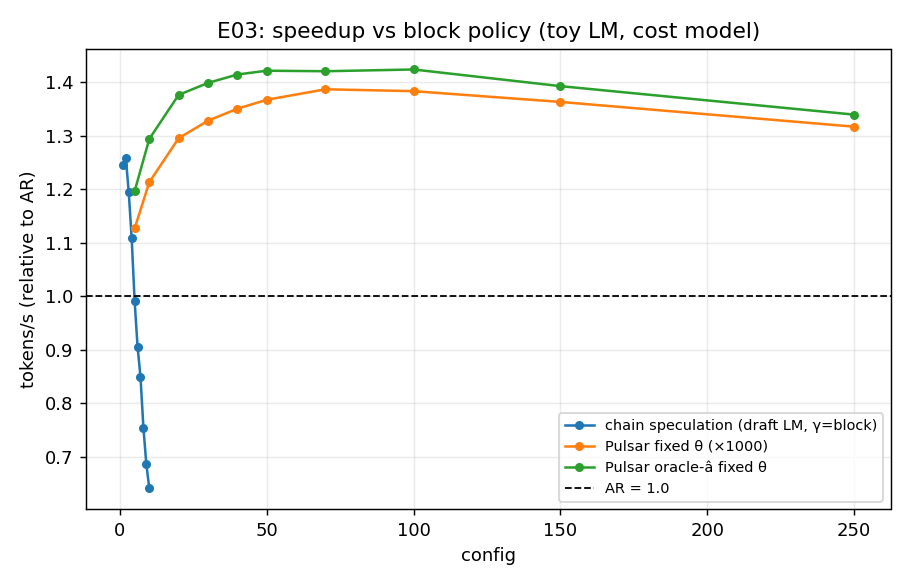
\includegraphics[width=.49\textwidth]{fig_e03_sweep.png}\hfill
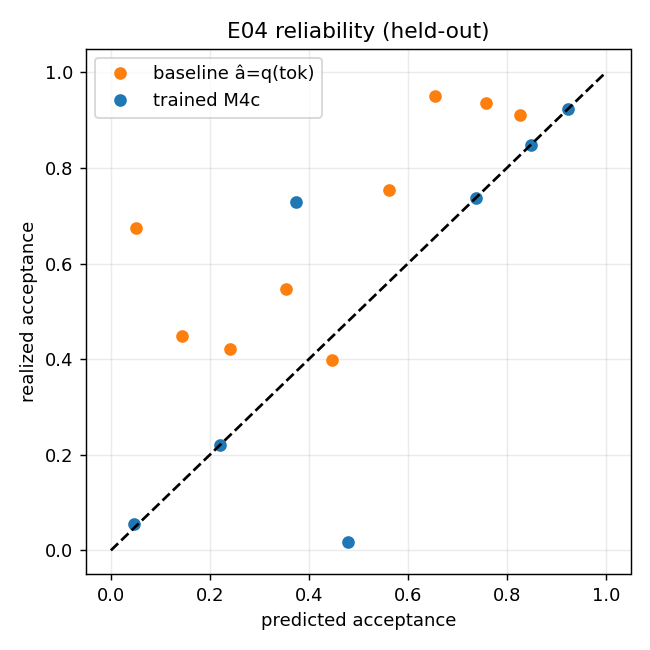
\includegraphics[width=.49\textwidth]{fig_e04_reliability.png}\\[4pt]
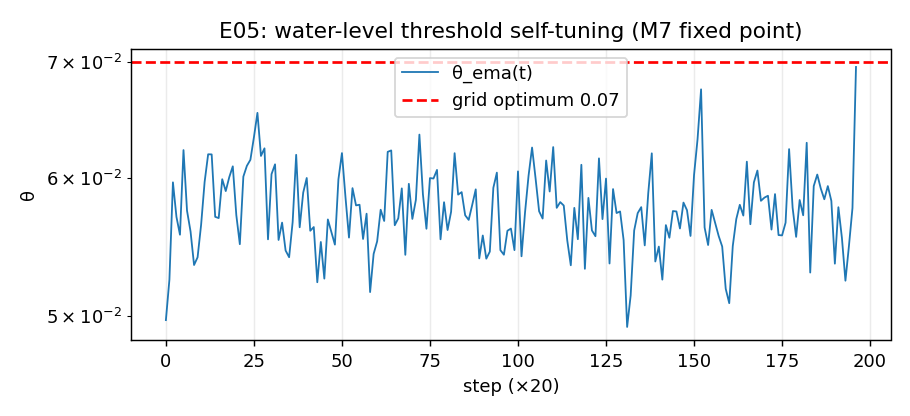
\includegraphics[width=.49\textwidth]{fig_e05_theta.png}\hfill
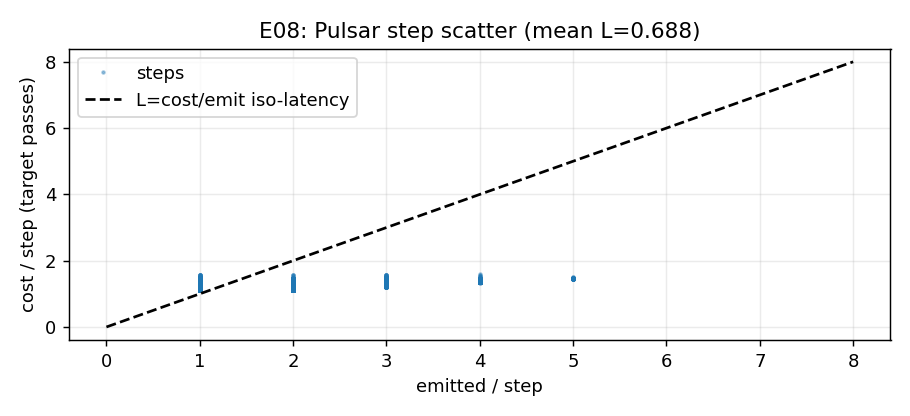
\includegraphics[width=.49\textwidth]{fig_e08_scatter.png}\\[4pt]
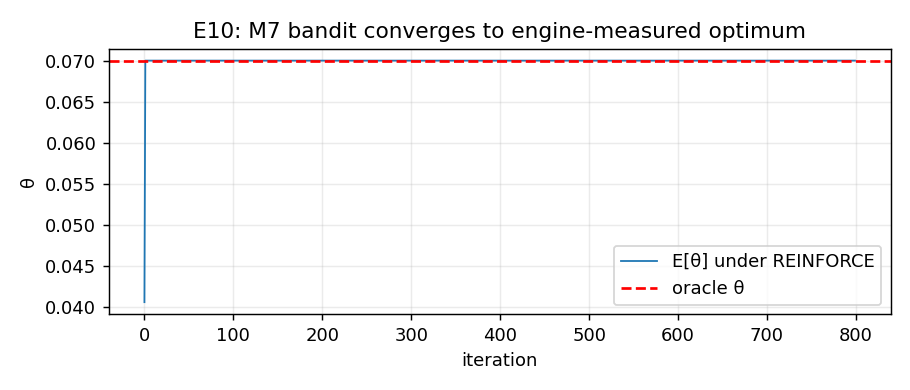
\includegraphics[width=.49\textwidth]{fig_e10_reinforce.png}\hfill
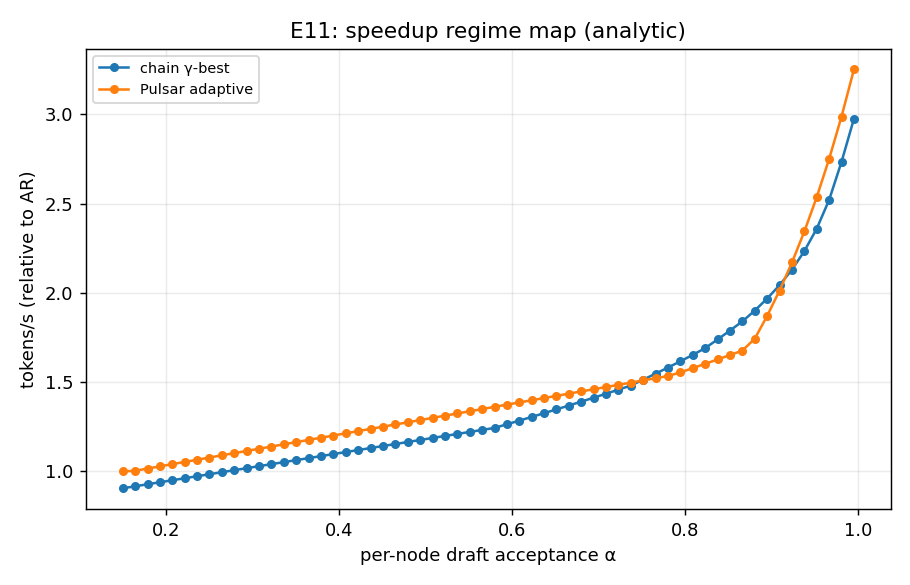
\includegraphics[width=.49\textwidth]{fig_e11_regime.png}
\caption{Top: block-policy sweeps; M4c reliability (held-out).
Middle: $\theta$ fixed point; per-step cost/yield scatter.
Bottom: M7 bandit; analytic regime map.}
\end{figure}

\section{Practitioner specification}
\label{sec:practice}
\textbf{Loop (vLLM/SGLang-style).}
(1) one hidden-state pass $\to$ head rows for the frontier layer (batched ---
breadth is one row; EAGLE-style feature drafting drops into M1);
(2) M4c scores, water-level expansion, top-$B$ per node, budget
$N\approx64$--$96$;
(3) tree-attention verification over the kept subtree;
(4) fall-through descent against the verifier table;
(5) commit $+$ bonus.
Training M4c: log (features, $\min(1,p/q)$) for \emph{all} children of
expanded nodes (anti-censoring), soft BCE, then PAVA isotonic.
Tuning M7: $\theta_{\text{mult}}=2.5$, EMA $0.05$ start; bandit if
non-stationary.
Numerics: log-space policy softmax with delta fallback; residual renorm
guard; $\hat a\in[10^{-6},1]$; $\theta$ floor.
What breaks first in production: assumed cost constants (measure them --- the
$\S\ref{sec:cost}$ formulas are your regression targets); selection-biased
labels as $\theta$ rises; batch $>1$ (shared rows shrink $c_{v1}$; rerun
E03-style sweeps on measured profiles); sampling-time top-$p$/top-$k$
truncation of $p$ (re-derive Thm~\ref{thm:exact} against the truncated law,
or disable truncation under Pulsar).

\section{Discussion}
\textbf{Metaphor boundary.} Load-bearing borrowings are exactly three:
rotor-sweep stratification (T06), pulse thresholds as fixed points
(T03/T05), beamed rare-dense-timed emission. Quantum vocabulary is confined
to diagonal $\rho$ and Born weights; no interference exists or is needed.
\textbf{Why M4c is the only trainable surface:} speed is monotone in
acceptance (head quality) and threshold calibration; verifier labels are
free and abundant, so gradients exist exactly there --- and
Theorem~\ref{thm:exact} makes unbounded training of that surface safe.
\textbf{Projections at published operating points:} Medusa-class
($\alpha\!\approx\!.75$, $c\!\approx\!.02$, $\gamma{=}4$):
$S\approx2.63$ (reported $2.2$--$2.8$); EAGLE-3-class
($\alpha\!\approx\!.88$, $c\!\approx\!.03$, $\gamma{=}8$): $S\approx6.05$
(reported up to $6.5$). Pulsar's deltas at such points: fall-through
$+29\%$ wherever tree sampling is used; adaptivity worth most under
$\mathrm{Var}(\alpha)$ (here $+10\%$; near zero when $\alpha$ is flat ---
measured, not oversold); clock bound and drift robustness are new in family.
\textbf{Limitations.} cost-model (not GPU wall-clock) speedups on a Markov
testbed; $V=20$; tail-bin calibration ceiling; 1-D bandit action space;
truncation interaction; energy unmeasured.
\textbf{Next.} CUDA tree-attention kernel re-running the whole harness on
\emph{measured} costs; lattice fields (Möbius-corrected $A$, conjectured to
preserve Thm~\ref{thm:water}); M4c on target hidden states; multi-sequence
joint fields with per-sequence $\theta$; adversarial-$\hat a$ studies (exact
outputs; how much speed can an attacker take?).

\section{Stage 6: bounded Transformers backend study}
The falsifiable empirical hypothesis is conditional: under a specified
inference backend and measured cost profile, a draft-confidence scheduler for
exact bounded trees improves held-out emitted tokens/s over a tuning-selected
fixed tree only when its paired 95\% confidence interval has a positive lower
bound. The adapter uses Transformers 4.46.3 with distilgpt2 as target and
sshleifer/tiny-gpt2 as draft, a shared 50,257-token GPT-2 tokenizer,
temperature-1 softmax, and a fixed 24-token horizon. EOS is ordinary. Timed
work includes prompt prefill, proposal/tree expansion, target evaluation,
verification, KV cache creation/commit, and output bookkeeping; model loading
is excluded.

Actual target and draft rows passed the Stage 1 pointwise identity over the
entire vocabulary on three held-out contexts. Maximum absolute error was
$1.08\cdot10^{-19}$; grouped empirical TV (32 largest target probabilities
plus OTHER) was 0.0116--0.0139 over 20,000 verifier samples per context. The
audited target-draft TV was high, 0.892--0.967.

\begin{center}
\begin{tabular}{lr}
\toprule
Method & Tokens/s \\
\midrule
Autoregressive target & 40.62 \\
Tuned chain ($\gamma=2$) & 15.71 \\
Tuned fixed tree (depth 2, branch 1) & 10.98 \\
Draft-confidence tree & 11.17 \\
\bottomrule
\end{tabular}
\end{center}

Paired bootstrap versus fixed tree: chain +43.00\% [34.87\%, 50.79\%],
confidence tree +1.66\% [-6.71\%, +10.01\%]. Versus autoregression:
chain -61.33\% [-63.47\%, -59.40\%], fixed tree -72.96\%
[-74.82\%, -70.71\%], and confidence tree -72.51\%
[-74.49\%, -70.63\%].

Two prompts selected the tuning actions; three disjoint prompts with three
paired seeds each formed the held-out evaluation. Chain lengths were
$\gamma\in\{2,4,6\}$; tree actions were (2,1), (3,1), (3,2), and (4,2).
Every confidence bin selected the same tuning-best fixed action. The scheduler
throughput claim is therefore \textbf{not established}: the point estimate is
positive, but its 95\% lower bound is negative. Chain speculation beat the
fixed-tree implementation, while both lost to autoregression on this profile.
This is a compact CPU experiment with three held-out prompt clusters and
level-batched full-context target rows, not a fused tree-attention kernel or a
general serving claim. The rotor/quantum framing is not part of the measured
algorithm. Stage 5 remains closed with its throughput gate unmet.

\section{Conclusion}
Pulsar specifies exact verification and scheduling contracts, but a correctness
guarantee is not a throughput guarantee. The frozen theory and toy-workload
results validate the stated probability and cost-model claims; they do not
establish neural-model serving speed. In the Stage 6 CPU integration, exactness
passed, while the confidence scheduler failed to establish a gain over the
fixed tree under the predeclared paired-interval criterion. Autoregression was
fastest; tuned chain speculation beat the fixed tree but both were slower than
autoregression. The defensible conclusion is a verified sampling adapter and a
bounded negative/inconclusive scheduler result---not a demonstrated
general-purpose acceleration. The next falsifiable step is to measure a
better-matched backend/model cost profile without reusing held-out prompts for
policy selection.

\appendix
\section{Full proofs}
\textbf{A.1 (Thm~\ref{thm:exact}, sequential form).} Induction on accepted
prefix: conditional on the prefix, the next position runs the pointwise
identity of \S\ref{sec:exact} with $\pi=\pi_u$; the policy may depend on
everything except the current coin; the residual branch terminates the walk
and its token law is $p$; the bonus row is sampled from the same pass,
independent of all coins. Chain $\Rightarrow$ tree $\Rightarrow$ arbitrary
prefix-closed fields with per-node policies. $\hfill\square$
\textbf{A.2 (Cor.~\ref{cor:yield}).} $P(X\ge k)=\prod_{j\le k}\alpha_j$ by
coin independence; $\mathbb E[X]=\sum_k P(X\ge k)$; geometric sum for the
uniform case. $\square$
\textbf{A.3 (Thm~\ref{thm:water}, trees).} Order all candidate nodes by
decreasing $A$; prefix-closure is automatic ($A$ decreases along paths).
Adding node $w$ to a set with state $(T,C)$ flips the sign of $C/T$ iff
$A_w < d\,T/C$; while adds are accepted $T/C$ is nondecreasing and the next
$A$ is smaller, so the condition crosses once; greedy = global optimum;
the threshold is the fixed point. Exhaustive check: slack
$\le3.4\cdot10^{-16}$. $\square$
\textbf{A.4} Continuous FOC for $S(H)$:
$\alpha^H\ln\alpha\,(1+cH)=c\,\tau(H)$ after clearing denominators;
solved by golden section (no elementary closed form; Lambert-$W$ applies
asymptotically). $\square$
\textbf{A.5 (stratification)} classical without-replacement variance;
round-robin realizes it exactly for $n\le N$. Row-stochastic mixing
preserves $\sum_u\psi$; the circulant acts as identity on
$\mathbf 1$ and $(1-\varepsilon)$ on the orthogonal complement. $\square$

\section{Interface contracts (as implemented)}
\begin{lstlisting}[style=code]
M1: (ctx, H_max, B) -> field{tok,par,dep,logq,psi,A,c2,c3}[nN]
M4c: X[nN,6] -> ahat in (0,1]          # draft-side features only
M4b: theta -> kept = {u : A[u] >= theta}  # prefix-closed by monotonicity
M4d: kept tree, pi_u -> path (sequential policy draw)
M3 : (path rows p, pi) -> emitted block (accept min(1,p/pi); residual norm((p-pi)+))
M6 : work(cycle) <= c_head*levels + c_tick*ceil(N/B_t) + 1 + c_v1*N
M7 : L_ema (or bandit state) -> theta ; verifier logs -> M4c supervision
\end{lstlisting}

\section{Reproduction}
\begin{lstlisting}[style=code]
python3 verification/theory_checks.py              # 11/11 expected
python3 verification/experiments/run_all.py  # 21/21; writes
   # results.json, figures, cpp/inputs/model.bin
cd cpp && make && ./pulsar_test inputs/model.bin   # PULSAR_TEST: PASS
python3 verification/experiments/test_stage6_transformers.py
python3 verification/experiments/run_stage6_transformers.py
\end{lstlisting}
Environment: Python 3.13, NumPy 2.3, SciPy 1.17 (tests only), g++ (C++17,
-O2 -march=native). Deterministic seeds; wall time ~4 minutes total.

\end{document}
